\subsection{Design one}
\label{design1}
This design revolves around the user being able to customize almost everything. The design therefore aims to be very flexible, and to accommodate almost every situation. The design of this system is structured with the following overview:

\begin{itemize}
\item user created wheel with attached stickers for camera registration and detection which will be utilized to accommodate several controller functionalities.
\item Additional gestures, not utilizing the wheel, which will accommodate controller functionalities.
\item Several possibilities to alter the specified gestures and functionalities to the users preferences. 
\end{itemize}


\subsubsection*{Description}
The user in this design will be given 3 or more stickers of different colours. See figure \ref{fig:wheel}. In this example, a red, green and a blue sticker are used, but since the design is so customizable, the user should be given the ability to choose colours him/herself. The user can also make the stickers themselves, in which case the product would be completely free for the user.


\begin{figure}[!htbp]
\centering
\subfigure[example sticker configuration.]{\label{fig:design11}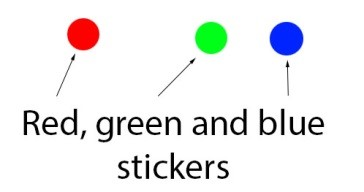
\includegraphics[scale=1]{Design11}}
\subfigure[Object for steering with stickers on.]{\label{fig:design12}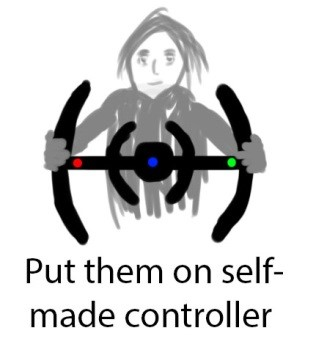
\includegraphics[scale=1]{Design12}}
\caption{Sticker configuration.}\label{fig:wheel}
\end{figure}

The user then places these stickers on some object he/she would like to use as a mean of controlling a vehicle inside a game. In this example, the stickers are placed on a steering wheel, which could be cut out from cardboard.

\begin{figure}[!htbp]
\centering
\subfigure[example of what the menu for steering could look like.]{\label{fig:design14}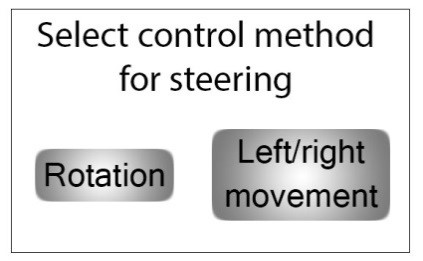
\includegraphics[scale=1]{Design14}}
\subfigure[example of what the menu for acceleration could look like.]{\label{fig:design13}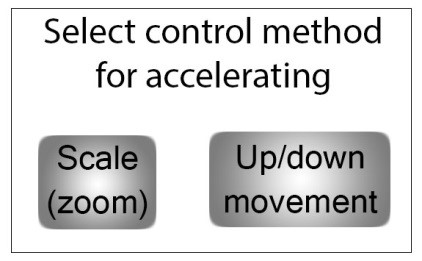
\includegraphics[scale=1]{Design13}}
\caption{Menu examples.}\label{fig:select}
\end{figure}

The user then picks how he/she would like to use the object for steering. Only two options are listed in this example, but more could be added, including ways of customizing the control method e.g., choosing how much you should be able to rotate the controller before reaching the maximum turning speed. See figure \ref{fig:select}.
\bigskip

Customization is also allowed for acceleration in which case the user can choose between moving the controller closer or further away from the camera, moving the controller up and down, or moving one hand up or down separately from the steering wheel. 
The acceleration itself would simply change between max acceleration and no acceleration at all (depending on the input from the camera), or acceleration, no acceleration, and braking, for simplicity. A separate sticker placed inside one’s hand can be used for braking, if it is needed to brake and use the speeder at the same time.
\bigskip

Gear shifting can be set up by being the “opposite” of controlling the speed. So if the user chooses to use up/down movement of the controller for speed, the user can use his/her free hand to separately control the gear shift. If the user holds their hand, with stickers attached, high, it would change the gear up, if the user holds it low, change the gear down, and if it’s in the center area, do not change gear. See figure \ref{fig:design15} for example of rotation, gear shifting would be done by releasing one hand from the steering wheel and use that for changing gear.

\begin{figure}[!htbp]
\centering
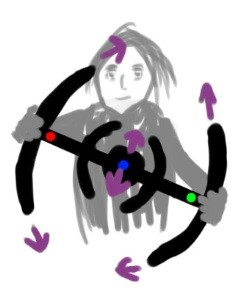
\includegraphics[scale=1]{Design15}
\caption{Controller in use.}
\label{fig:design15}
\end{figure}

To implement an extra action such as using power-ups or something similar, the opposite
of the steering control method could be used. If the user is using rotation for steering,
left/right movement could be used for extra action functionalities, and vice versa if the user
chose left/right movement for steering. After everything is set up, the user now has his/her own custom-made controller, unlike any other. He/she can use it to control things inside games (although this is optimized for vehicle games), only needing a webcam to pick up the colours, and a computer.
\bigskip

As a prototype using this design, the control methods that are to be implemented are listed below in categories of what actions the methods are used for. As mentioned the user will choose between one of the methods listed for each action. One method can be listed for two different actions, but if the user chooses one method for one action he/she can not choose it again for another action. The list is as follows:

\begin{itemize}
	\item Steering the car:
	\begin{itemize}
		\item Rotation – Tracking rotation movement of stickers placed on the controller.
		\item Left/right movement – Tracking stickers on the controller moving horizontally.
	\end{itemize}
	
	\item Acceleration \& braking:
	\begin{itemize}
		\item Up/down movement – Tracking vertical movement of the stickers.
		\item Forward/backward movement.
		\begin{itemize}
			\item Tracking change in distance between stickers on the controller.
			\item Tracking change in size of one sticker (or multiple).
		\end{itemize}
	\end{itemize}
	
	\item Gear shifting:
	\begin{itemize}
		\item Up/down movement – As above.
		\item Forward/backward movement – As above.
		\item Hand gesture, up/down movement – Tracking vertical movement of a sticker on a hand. Here the user must release the controller with the one hand.
	\end{itemize}
	
	\item Extra action:
	\begin{itemize}
		\item Rotation – As above.
		\item Left/right movement – As above
	\end{itemize}
\end{itemize}
\bigskip

\subsubsection*{Compared to the FPS and List of Requirements}
The FPS is focused on creating a cheap alternative to already existing vehicle controllers. This design not only creates a solution that needs nothing else than a standard laptop, it also lets the user specify and choose almost every aspect of controlling, and lets them create their own controller. It is not even necessary to make a controller; the user can paint their hands and use them instead if they want.

Compared to the list of requirements, this design fulfills everything but the ability to brake while accelerating. In the example explained, it also does not fulfil the ability for extra action buttons. However the design can be made more complete to allow such control methods, without the need of additional purchases, such as buttons, by adding customization options to the user.


\pagebreak[2]
\subsubsection*{Pros and Cons}
Pros:
\begin{itemize}
\item It is free of cost, provided the user has a computer and webcam.
\item Potentially adds an infinite number of customization options.
\item It is not limited to a single game.
	\end{itemize}
Cons:
\begin{itemize}
\item The amount of setting-combinations could be complicated for the user.
\item It could be hard to make.
\end{itemize}

\subsubsection*{Software specifications}
In order to conduct tracking, colour tracking can be used as described earlier. This method would likely be the simplest and easiest way to utilize tracking through a standard web cam. However, there is several limitations to colour tracking such as colour usage which might be worn by the user and therefore limits the usage. Additionally, lighting and other room conditions can alter the usability of colour recognition.

Potentially, pattern recognition or template matching could be an alternative to colour recognition, diminishing the specified complications. In this case, the surrounding environment is not compromised in terms of colour.

\pagebreak[2]